\section{Simulator Evaluation}

\subsection{Overall System}
\begin{enumerate}
	\item It works on other machines first run, (different machine different gpu). Verify it works on WSL?
\end{enumerate}

\subsection{Tracking System}
\subsubsection{Together}
\begin{enumerate}
	\item Draw a bell curve of latency. Don't forget to factor in the latency built into the camera. 
	\item Justify the downscaling, show that it's slow with no upscaling and downscaling even more offers negligible speed increases.  
	\item Mention lighting issues.
\end{enumerate}

\textcolor{red}{stop calling it latency it's the framerate}

\begin{figureBox}[label={fig:overall-latency}, width=1.0\linewidth]{Overall latency}
	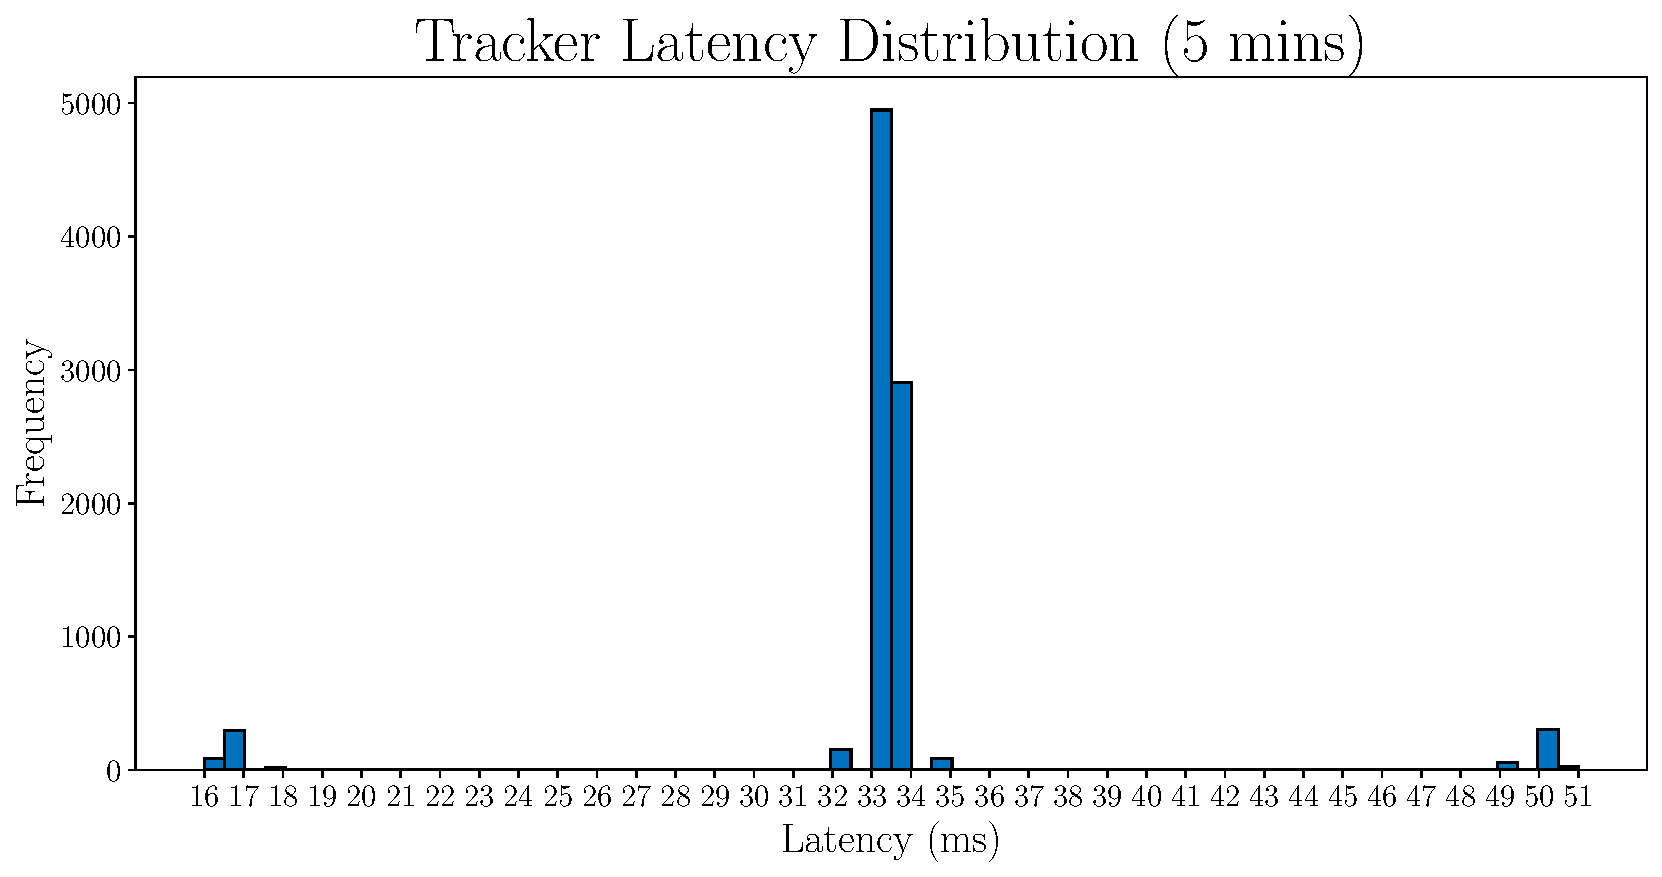
\includegraphics[width = 1.0\linewidth]{./evaluation/figures/overall-latency.pdf}
\end{figureBox}

As can be seen in Figure \ref{fig:overall-framerate}, the latency of the system is quite low. 90.83\% of the time the latency is between 30 and 35ms. There is what at first glance a strange phenomenon of a group of latencies at 16-18ms (4.46\%) and 49-51ms (4.39\%). I believe this is due to the framerate of the renderer, as it lazily converted on request it basically chunked to the nearest 1000/60 = 16.666.

We investigated downscaling the image to increase performance. We only found that downscaling it once was enough to get the performance we needed. Downscaling it further did not offer any significant performance increases and significantly decreased tracking quality. As can be seen in Figure \ref{fig:pydown}, the performance of the system increases noticeably between going from 2048 x 1536 to 1024 x 793 but reducing the resolution further does not provide any speed benefit at all as we are already running at 30fps which is the cameras refresh rate..

\begin{figureBox}[label={fig:pydown}, width=1.0\linewidth]{Comparing Resolutions}
	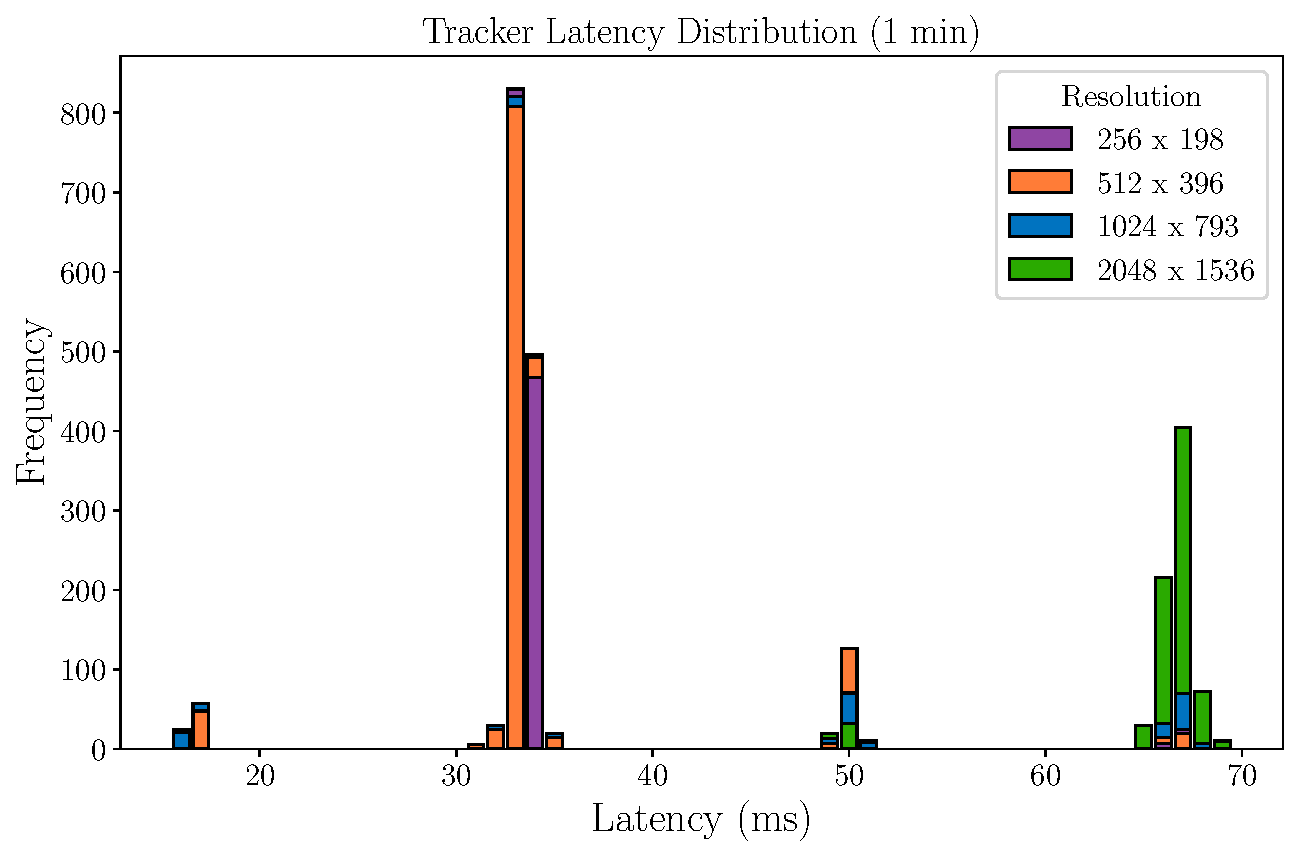
\includegraphics[width = 1.0\linewidth]{./evaluation/figures/pydown.pdf}
\end{figureBox}


\subsubsection{Head Tracking}
\begin{enumerate}
	\item Estimate throughput via logging (unique points). Draw a bell curve like graph of the time between each result from the tracker.
	\item Measure accuracy by moving head around and seeing how often it loses track at different distances. While facing camera. Test with glasses on?
	\item Measure the angle of the head where the tracker stops working.  
\end{enumerate}

\subsubsection{Hand tracking}
\begin{enumerate}
	\item Estimate throughput via logging (unique points). Draw a bell curve like graph of the time between each result from the tracker.
	\item Measure accuracy by moving head around and seeing how often it loses track at different distances. Change hand orientations
	\item Mention occlusion issue. 
	\item Wall vs no wall issue. 
	\item The colour of the screen also affects the hand tracker. 
\end{enumerate}

\subsection{Renderer}
\begin{enumerate}
	\item Reconstruct real life item, compare photos of item from different angles. 
	\item Get framerate?
\end{enumerate}